
\documentclass{report}

\usepackage[utf8]{inputenc}
\usepackage[italian]{babel}
\usepackage{import}
\usepackage{todonotes}
\usepackage{color}
\usepackage{rotating}
\usepackage[hidelinks]{hyperref}
\usepackage{url}
\usepackage{pdfpages}
\usepackage{siunitx}
\usepackage{pdflscape}
\usepackage{subfig}
\usepackage[euler]{textgreek}
\usepackage{mhchem}

\usepackage{enumerate} 
\usepackage{amsmath}
\usepackage{amsfonts}

\usepackage[signatures,swapnames,sans]{frontespizio}

\usepackage{geometry}
\geometry{portrait, margin=3cm}
\usepackage{siunitx}
\usepackage{booktabs}

\renewcommand*\figurename{Figura}

\newcommand{\sub}[1]{\textsubscript{#1}}
\newcommand{\super}[1]{\textsuperscript{#1}}
\newcommand{\parallelsum}{\mathbin{\!/\mkern-5mu/\!}}

\newcommand{\Fig}[0]{Fig.}

\usepackage{titlesec}

\titleformat{\chapter}{\normalfont\huge}{}{20pt}{\huge\bfseries}

\linespread{1.3}


%% COMANDI UTILI
%\begin{table}[h]
%	\centering
%	\begin{tabular}{|c|c|c|}
%	\cline{2-3} 
%	\multicolumn{1}{c|}{} & \textbf{Valore nominale} & \textbf{Valore misurato}\\ 
%		%\hline
%		%{} & \textbf{Valore nominale} & \textbf{Valore misurato} \\ 
%		\hline
%		$\mathbf{R_1}$ & \SI{18}{k\ohm} & \SI{17.977}{k\ohm} \\ 
%		\hline
%		$\mathbf{R_2}$& \SI{1.8}{k\ohm} & \SI{1.815}{k\ohm} \\ 
%		\hline
%	\end{tabular}
%\caption{Misure delle resistenze utilizzate per il circuito.}
%\label{table:mis_res}
%\end{table}
%\begin{figure}[h!]
%\centering
%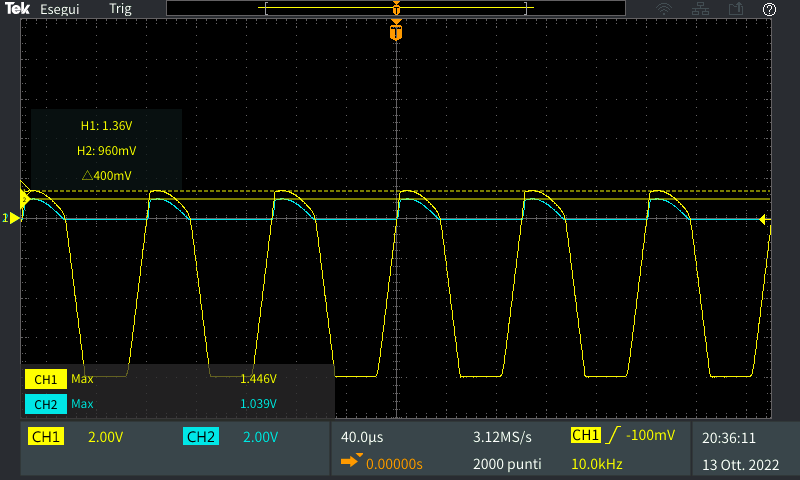
\includegraphics[height=6.5cm]{immagini/TEK00018}\\(a)\\[1ex]
%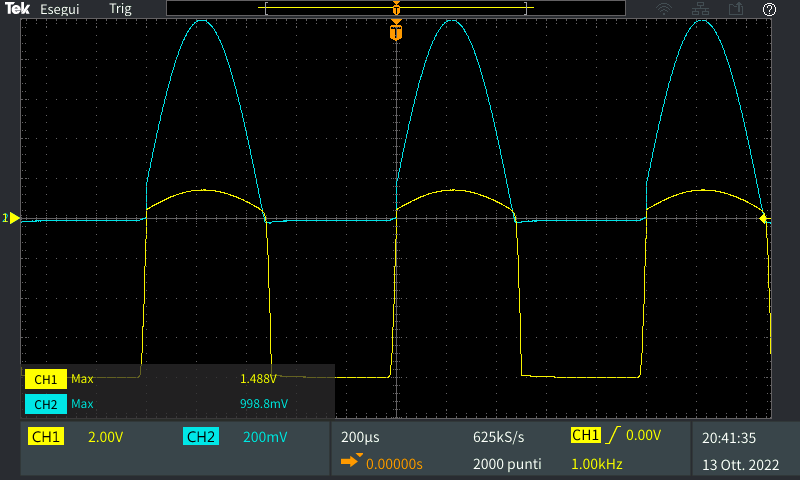
\includegraphics[height=6.5cm]{immagini/TEK00019}\\(b)
%\caption{Risposta del circuito con accoppiamento DC (a) e accoppiamento AC (b).}
%	\label{figura:accopp}
%\end{figure}

\begin{document}
\addtocounter{chapter}{+1}
	\begin{frontespizio}
		\Margini{3cm}{3cm}{3cm}{3cm}
		\Universita{Bergamo}
		\Logo[43.332mm]{unibg-mark}
		\Divisione{Scuola di Ingegneria}
		\Corso[Laurea Magistrale]{Ingegneria Informatica}
		\Titolo{Laboratorio di Elettronica}
		\Sottotitolo{Relazione esperienza di laboratorio 2}
		\Punteggiatura{}
		\NRelatore{Prof.}{Prof.}
		\Relatore{Luigi Gaioni}
		\Candidato[1058231]{Giulia Allievi}
		\Candidato[1059640]{Martina Fanton}
		\Annoaccademico{2022--2023}
		\begin{Preambolo*}
			\usepackage[italian]{babel}
			\usepackage[T1]{fontenc}
			\usepackage[utf8]{inputenc}
			\usepackage{microtype}
			\usepackage{lmodern}
			\graphicspath{{img/}}
			
			\renewcommand{\frontinstitutionfont}{\fontsize{14}{17}\bfseries\scshape}
			\renewcommand{\fronttitlefont}{\fontsize{17}{21}\bfseries\scshape}
			\renewcommand{\frontfootfont}{\fontsize{12}{14}\bfseries\scshape}
		\end{Preambolo*}
	\end{frontespizio}

%----------------------------------------------------------------------------------------
%	PAGINA BIANCA
%----------------------------------------------------------------------------------------
\newpage
\null
\thispagestyle{empty}
\newpage

%----------------------------------------------------------------------------------------
%	INTRO
%----------------------------------------------------------------------------------------
% Ho cambiato la struttura per questa relazione così rimane tutto nominato con il numero 2
\chapter{Relazione attività di laboratorio 2}
\section{Circuito 1: raddrizzatore}
\subsection{Schema del circuito e Funzione di Trasferimento}
\begin{figure}[h]
	\centering
	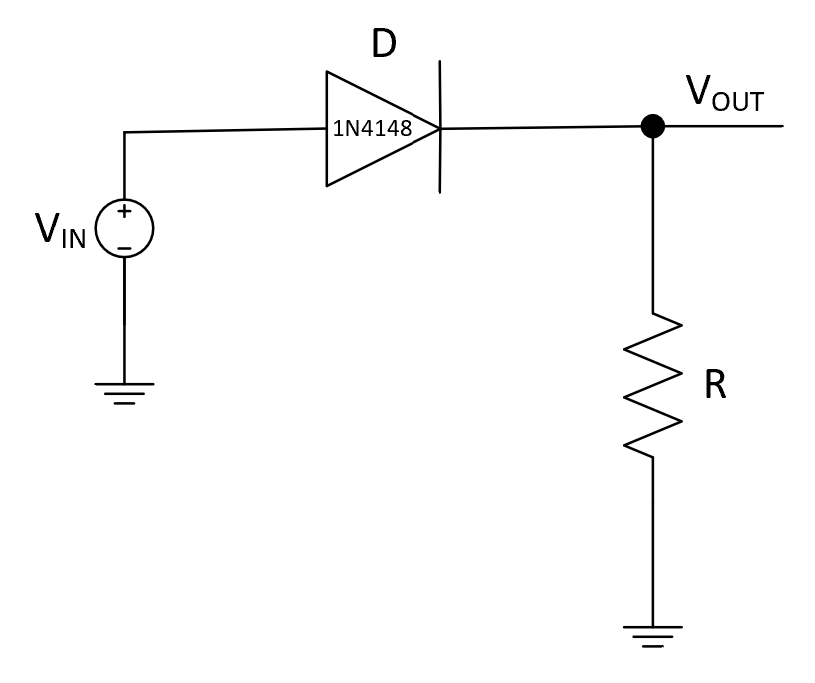
\includegraphics[height=6.5cm]{immagini/schema1}
	\caption{Schema del circuito.}
	\label{figura:schema1}
\end{figure}
\subsection{Analisi e dati sperimentali}

\newpage
\section{Circuito 2: raddrizzatore}
\subsection{Schema del circuito e Funzione di Trasferimento}
\begin{figure}[h]
	\centering
	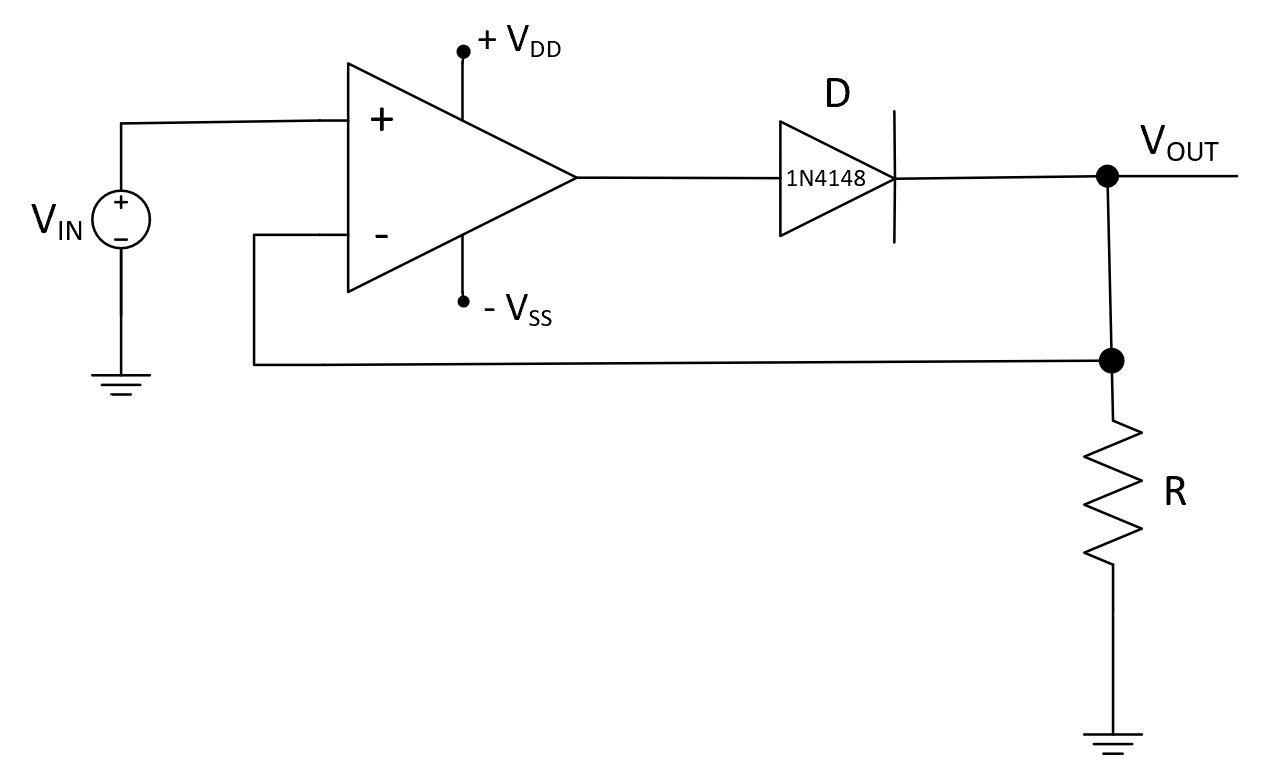
\includegraphics[height=6.5cm]{immagini/schema2}
	\caption{Schema del circuito.}
	\label{figura:schema2}
\end{figure}
\subsection{Analisi e dati sperimentali}

\newpage
\section{Circuito 3: raddrizzatore a doppia semionda}
\subsection{Schema del circuito e Funzione di Trasferimento}
In questo circuito (come mostrato nella figura \ref{figura:schema3}), a differenza dei precedenti due, sono presenti due diodi: il primo è collegato all'uscita dell'OPAMP, mentre il secondo è posizionato nella retroazione del circuito.u
\\Inoltre il raddrizzatore a doppia semionda presenta due retroazioni negative e in particolare quella costituita dalla sola resistenza R è sempre chiusa permettendo al circuito in esame di non operare in anello aperto.
\\In aggiunta l'amplificatore si trova in configurazione invertente e per la presenza di resistenze equivalenti presenta un guadagno pari a -1.
\begin{figure}[h]
	\centering
	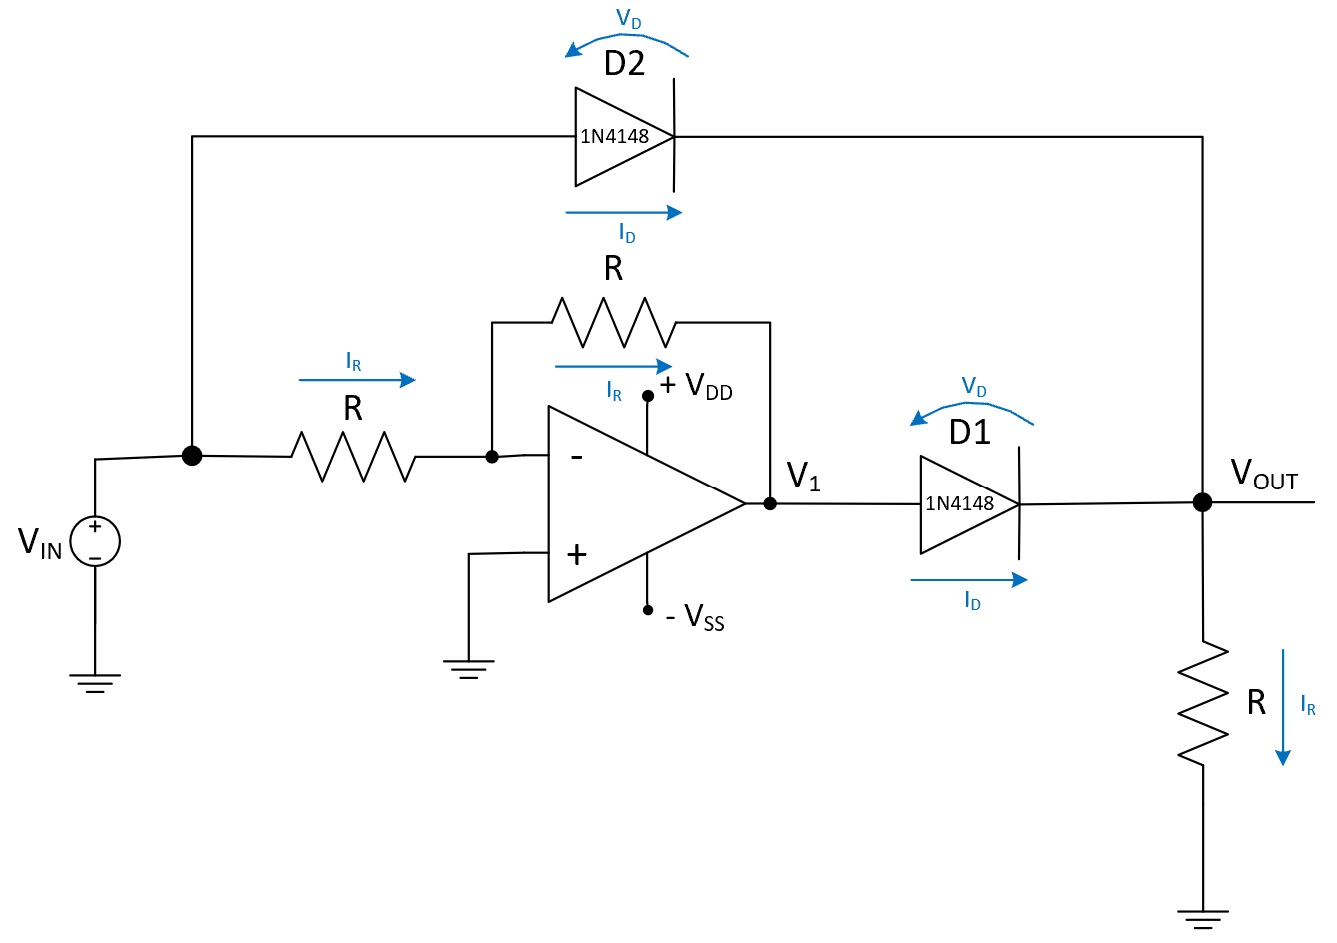
\includegraphics[height=6.5cm]{immagini/schema3}
	\caption{Schema del circuito.}
	\label{figura:schema3}
\end{figure}
\\La Funzione di trasferimento corrispondente a questo circuito è:
% INSERIRE FDT
\subsection{Analisi e dati sperimentali}
Come primo passo per la costruzione del circuito, sono stati misurati i valori dei componenti che verranno utilizzati. In particolare abbiamo scelto tre resistenze da \SI{12}{k\ohm}. Le loro misure sono state riportate nella tabella \ref{table:mis_res3}.
\begin{table}[h]
	\centering
	\begin{tabular}{|c|c|c|}
		\cline{2-3} 
		\multicolumn{1}{c|}{} & \textbf{Valore nominale} & \textbf{Valore misurato}\\ 
		\hline
		$\mathbf{R_1}$ & \SI{12}{k\ohm} & \SI{11.802}{k\ohm} \\ 
		\hline
		$\mathbf{R_2}$ & \SI{12}{k\ohm} & \SI{11.947}{k\ohm} \\ 
		\hline
		$\mathbf{R_3}$ & \SI{12}{k\ohm} & \SI{11.885}{k\ohm} \\ 
		\hline
	\end{tabular}
	\caption{Misure delle resistenze utilizzate per il circuito.}
	\label{table:mis_res3}
\end{table}
\\Una volta realizzato il circuito sulla breadboard, sono poi state effettuate delle misure (presenti nella tabella \ref{table:misure3}) dei valori di tensione nei vari nodi del circuito considerando i segnali in ingresso e in uscita a diverse frequenze (quelle considerate sono state: \SI{1}{k\hertz}, \SI{10}{k\hertz}, \SI{100}{k\hertz} e \SI{400}{k\hertz}).
\begin{table}[h!]
	\centering
	\begin{tabular}{|c|c|c|c|}
		\hline
		\textbf{Frequenza} & \boldmath$\displaystyle\mathrm{{V_{1}}}$\textbf{/}\boldmath$\displaystyle\mathrm{{V_{PP,in}}}$ & \boldmath$\displaystyle\mathrm{{V_{PP,out}}}$\textbf{[V]}\ & \boldmath$\Delta$\textbf{V [V]}\\
		\hline
		1 kHz & 0.980 & 0.520 & 0.460\\
		\hline
		10 kHz & 0.960 & 0.520 & 0.440\\
		\hline
		100 kHz & 0.980 & 0.520 & 0.460\\
		\hline
		400 kHz & 0.528 & 0.288 & 0.240\\
		\hline\end{tabular}
	\caption{Grandezze misurate ad ogni frequenza.}
	\label{table:misure3}
\end{table}
\\Per quanto riguarda la frequenza di \SI{1}{k\hertz}, come si può notare dalla figura \ref{figura:TEK00022}, i segnali presentano un andamento quasi ideale.
\\A questa frequenza si può anche notare la presenza di un offset tra la tensione in ingresso e quella in uscita, che risulta pari a \SI{0.460}{\volt}.
\begin{figure}[h]
	\centering
	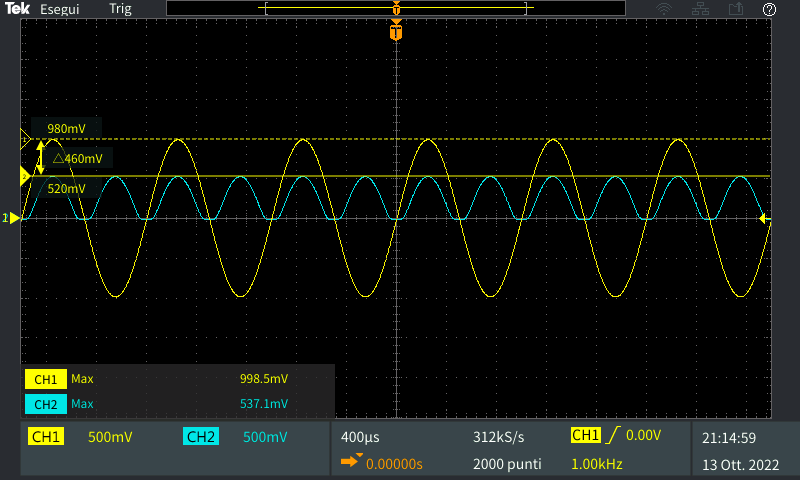
\includegraphics[height=6cm]{immagini/TEK00022}
	\caption{Segnali di $\mathbf{V_1}$ e di $\mathbf{V_out}$ con frequenza di \SI{1}{k\hertz}.}
	\label{figura:TEK00022}
\end{figure}
\\Invece se ad esempio si considera la frequenza da \SI{100}{k\hertz}, come si può notare dalla figura \ref{figura:TEK00025}, si può notare che i segnali presentano una curva più estesa nella fase di spegnimento del diodo rispetto a quella della fase di accensione. Questo andamento risulta ancora più accentuato nella figura \ref{figura:TEK00030} in cui la frequenza considerata è di \SI{400}{k\hertz}.
\begin{figure}[h]
	\centering
	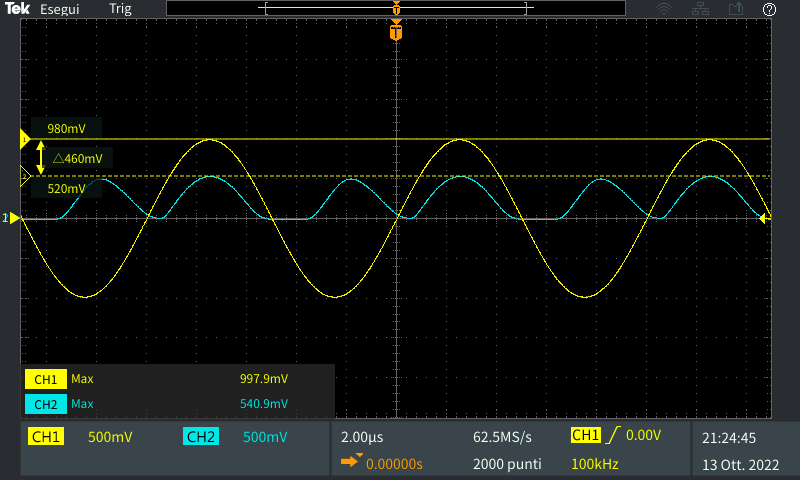
\includegraphics[height=6cm]{immagini/TEK00025}
	\caption{Segnali di $\mathbf{V_1}$ e di $\mathbf{V_out}$ con frequenza di \SI{100}{k\hertz}.}
	\label{figura:TEK00025}
\end{figure} 
\begin{figure}[h]
	\centering
	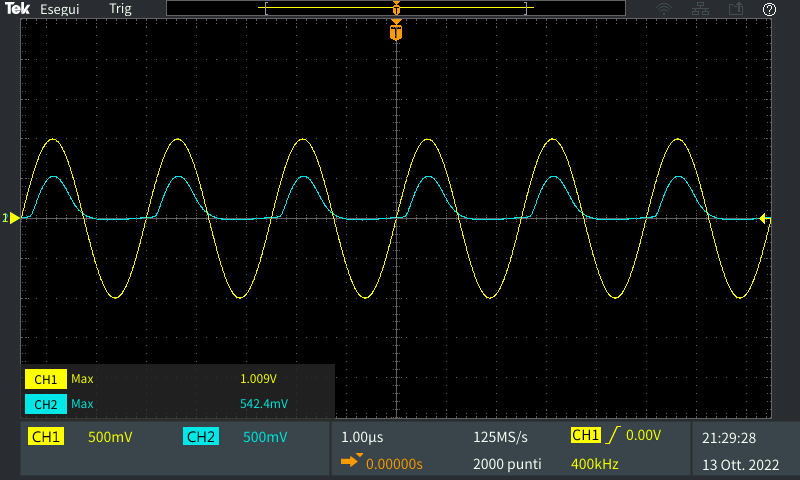
\includegraphics[height=6cm]{immagini/TEK00030}
	\caption{Segnali di $\mathbf{V_1}$ e di $\mathbf{V_out}$ con frequenza di \SI{400}{k\hertz}.}
	\label{figura:TEK00030}
\end{figure} 
\\Poi come si può notare dai grafici di questo circuito, il raddrizzatore a doppia semionda risolve il problema causato dallo swing della tensione $\mathbf{V_1}$ del secondo raddrizzatore analizzato. In questo modo la tensione in uscita all'OPAMP evita di raggiungere i valori delle alimentazioni dell'amplificatore stesso e di determinare proprio degli swing in tensione.

%----------------------------------------------------------------------------------------

\end{document}
